\section{Procesos desarrollados durante la práctica}
%\subsection*{Objetivos}
\begin{frame}{Objetivo general}%{Métodos}
    Proporcionar los conocimientos teóricos adquiridos en las sesiones académicas durante la formación universitaria en la Sub Gerencia de Obras y Desarrollo Urbano y Rural, específicamente en el área de Unidad de Obras y Equipo Mecánico.
\end{frame}

\begin{frame}{Objetivos específicos}
    \begin{itemize}
        \item Afianzar los conocimientos sobre la gestión pública, en concordancia con las directrices y normativas establecidas por la Municipalidad Distrital de Tamburco.
        \item Adquirir conocimientos en la elaboración de fichas técnicas con fondos asignados por el Ministerio de Economía y Finanzas en entidades gubernamentales.
        \item Ampliar y profundizar el dominio de software esencial en el campo de la ingeniería tales como son: AutoCAD 2021, Revit, AutoCAD Civil 3D, QGIS y Excel 2021 y Oracle Primavera P6 % En cuanto al análisis estructural, programas como ETABS y SAFE son fundamentales y dominarlos me permitirá realizar evaluaciones estructurales detalladas y precisas. 
        \item Asimilar conocimientos, experiencias y sugerencias.
     \end{itemize} 
\end{frame}
%%%%%%%%%%%%%%%%%%%%%%%%%%%%%%% SLIDE 2 %%%%%%%%%%%%%%%%%%%%%%%%%%%%%%%%%%
%\subsection*{Descripción}
\begin{frame}{Descripción del proyecto}
    La infraestructura vial en mención, está clasificada como vía nacional  PE 30S, las carreteras en el Perú se clasifican de acuerdo a 2 criterios: En función a su demanda de 400 - 2000 veh/día y en función a su orografía según menciona \cite[12]{MTC2018}, comunica las ciudades de Abancay y Cusco, constituido de pavimento flexible que a medida transcurre por zonas urbanas existen intersecciones con pavimentos rígidos.
\end{frame}

%%%%%%%%%%%%%%%%%%%%%%%%%%%%%%% SLIDE 3 %%%%%%%%%%%%%%%%%%%%%%%%%%%%%%%%%%
%\subsection*{Estado}
\begin{frame}{Estado situacional}
    \begin{enumerate}%[noitemsep]
		\item Intersección Av. Tupac Amaru  -  Av. Tamburco (KM: 775+44  -  775+74)
		\item Intersección Av. Tamburco  -  Jr. Señor de Exaltacion (KM: 774+67  -  775+03)
		\item Intersección Av. Tamburco  -  Coronel Gonzales (KM: 794+25  -  795+57)
		\item Intersección Av.Tamburco  -  14 de Septiembre (KM: 773+44  -  773+76.649)
		\item Av. Tamburco (KM: 776+51  -  776+65)
		\item Intersección Av. Tamburco  -  Calle Martinelli (KM: 766+51  -  766+64.14)
		\item Intersección Av. Tamburco  -  Prolon. Huancavelica (KM: 765+31  -  765+45.96)
		\item Intersección Av. Tamburco  -  Prolong. Nuñez (KM: 763+31  -  763+52.5870)
		\item Av. Tamburco (Grifo REPSOL) (KM: 762+43  -  763+00)
		\item Intersección Av. Tamburco  -  Av. Taracalle (KM:761+49.79  -  761+70.333)
	\end{enumerate}
\end{frame}

%%%%%%%%%%%%%%%%%%%%%%%%%%%%%%% SLIDE 4 %%%%%%%%%%%%%%%%%%%%%%%%%%%%%%%%%%
%\subsection*{Objetivos de la obra}
\begin{frame}{Objetivos específicos de la obra}
    \begin{enumerate}%[noitemsep]
		\item Mantener en óptimas condiciones la infraestructura vial, reparando baches y nivelando calles, implementar una señalización clara y eficaz que permita a los conductores anticipar a las condiciones de la vía.
		\item Reducir significativamente en los costos de mantenimiento de los vehículos disminuyendo el desgaste y la necesidad de reparaciones ocasionadas por condiciones adversas en las vías.
		\item Facilitar el flujo vehicular y así reducir la congestión vehicular.
		\item Reducir los niveles de contaminación y mejorar la calidad del aire en la ciudad de Tamburco.
	\end{enumerate}
\end{frame}

%%%%%%%%%%%%%%%%%%%%%%%%%%%%%%% SLIDE 5 %%%%%%%%%%%%%%%%%%%%%%%%%%%%%%%%%%
%\subsection*{}
    \begin{frame}{Ubicación del proyecto}%{Ubicación geográfica}
\begin{figure}[h]
\captionsetup{width=1\textwidth}
\centering
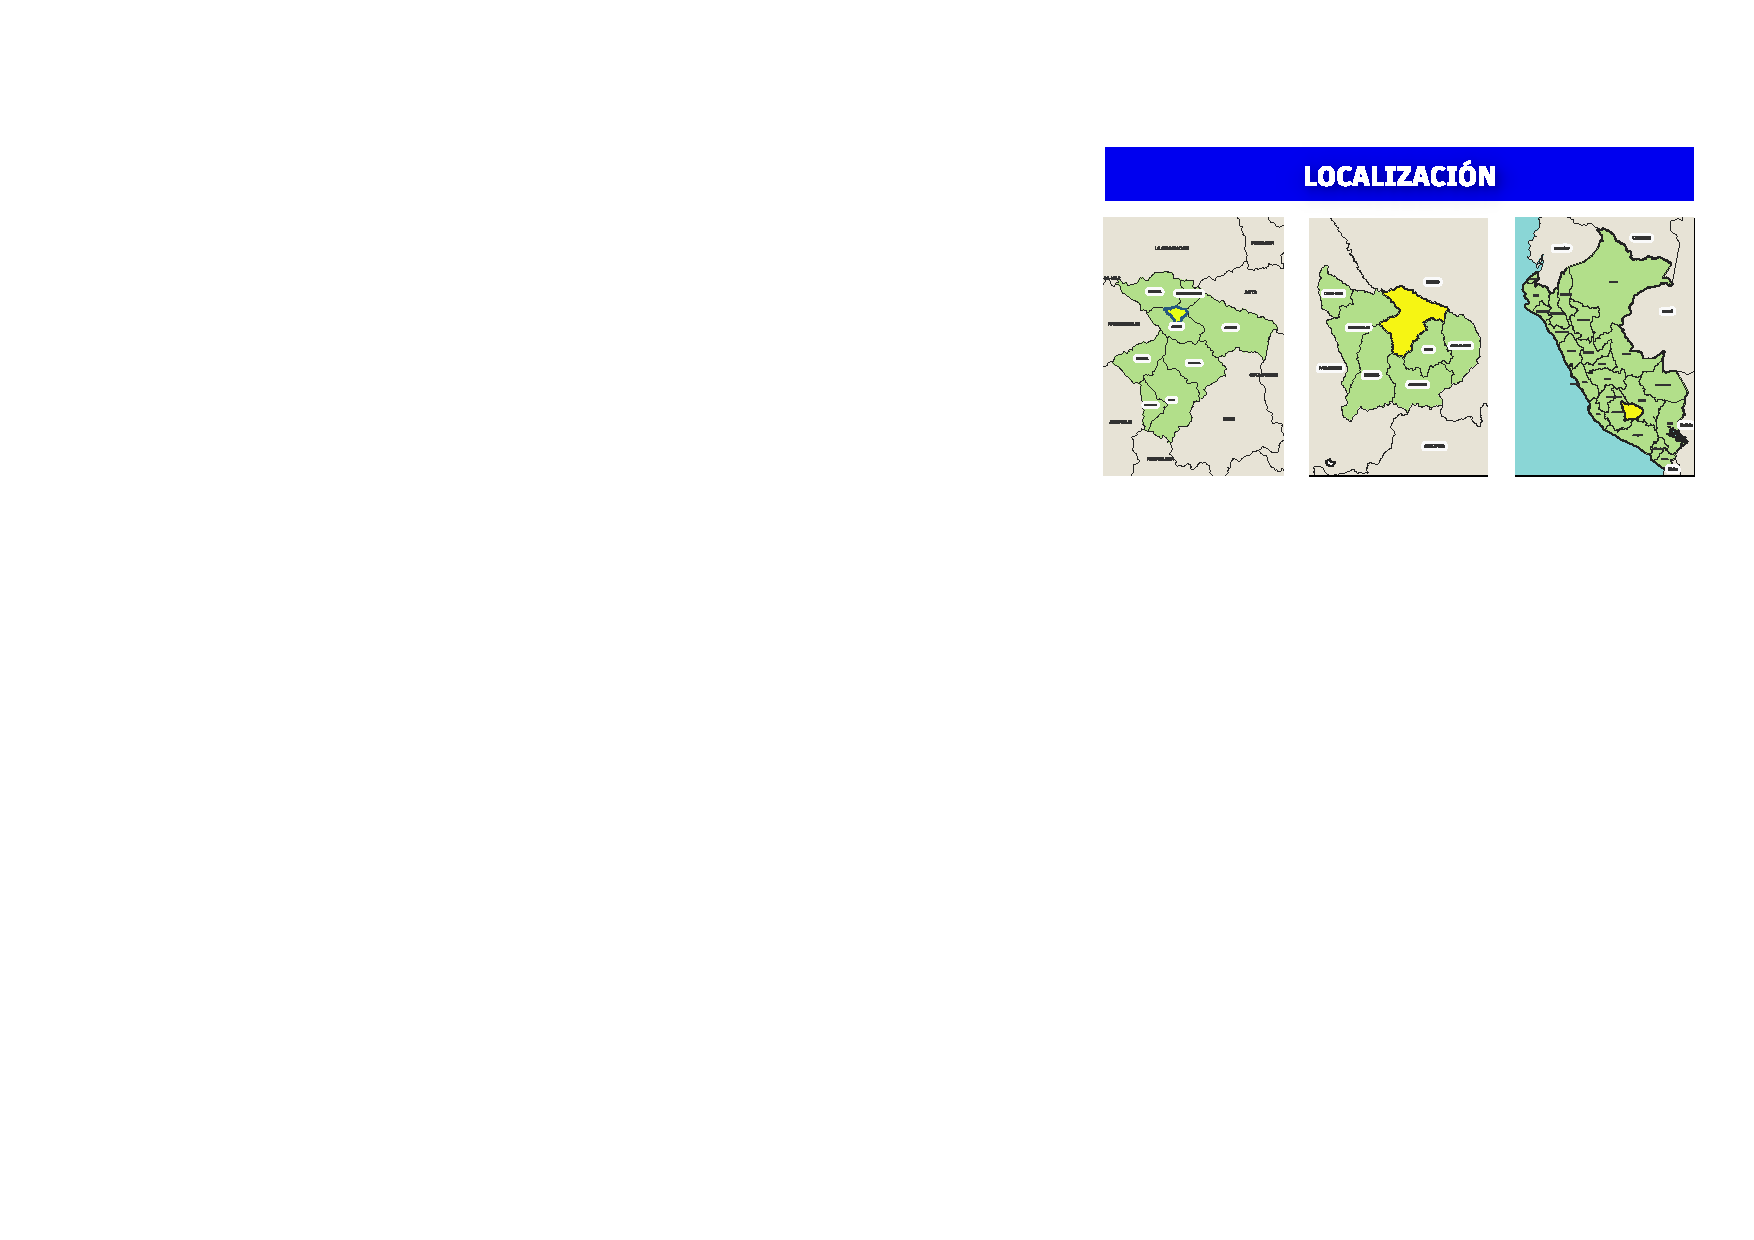
\includegraphics[width=0.65\textwidth]{2.3.pdf}
\caption[Ubicación del proyecto]{El proyecto está ubicado en la región de Apurínac, provincia de Abancay, distrito de Tamburco. Toda la infraestructura vial se denomina Avenida Tamburco}
\label{fig:etiqueta}
\end{figure}
    \end{frame}

%%%%%%%%%%%%%%%%%%%%%%%%%%%%%%% SLIDE 6 %%%%%%%%%%%%%%%%%%%%%%%%%%%%%%%%%%
%\subsection*{}
\begin{frame}{Especificaciones técnicas}%{Deficinión}
	\begin{block}{Definición}
		Son el conjunto detallado de características y requisitos técnicos que deben cumplir un producto, sistema o servicio.
	\end{block}
	\begin{block}{Normativas}
		\begin{itemize}
			\item \citetitle[]{MVCS2010} publicado por \cite[]{MVCS2010}
			\item \citetitle[]{MTC2013} publicado por \cite[]{MTC2013}
		\end{itemize}
	\end{block}
\end{frame}
%%%%%%%%%%%%%%%%%%%%%%%%%%%%%%% SLIDE 7 %%%%%%%%%%%%%%%%%%%%%%%%%%%%%%%%%%
\begin{frame}{Diseño de pavimentos rígidos}{Fórmula general de AASTHO}
	\begin{equation}
		\resizebox{\linewidth}{!}{$\log(W_{18}) = Z_{R} \cdot S_{0} + 7.35 \cdot \log(D+1) - 0.06 + \frac{ \log \left( \frac{\Delta PSI}{4.15 - 1.5} \right)}{\frac{1.624 \cdot 10^{7}}{(D+1)^{8.46}}} + (4.22 - 0.32 \cdot P_{t}) \cdot \log \left[ \frac{S'_{c} \cdot C_{d}(D^{0.75} - 1.132)}{215.63 \cdot \left[D^{0.75}- \frac{18.42}{\left[ \frac{E_{c}}{k} \right]^{0.25}} \right]} \right]$}
	\end{equation}
\end{frame}
%%%%%%%%%%%%%%%%%%%%%%%%%%%%%%% SLIDE 8 %%%%%%%%%%%%%%%%%%%%%%%%%%%%%%%%%%
\begin{frame}{Dónde:}
	%\begin{block}{Dónde:}
\begin{itemize}
	\item \(W_{18}\) = Número de cargas de 18 kips (80 kN) previstas 
	\item \(Z_{R} \) = Es el valor de Z (área bajo la curva de distribución) correspondiente a la curva estandarizada, para una confiabilidad R.
	\item \(S_{0} \) = Desvío estándar de todas las variables
	\item \(D\) = Espesor de la losa del pavimento en pulgadas 
	\item \(\Delta PSI\) = Pérdida de serviciabilidad prevista en el diseño
	\item \(P_{t}\) = Serviciabilidad final
	\item \(S'_{c}\) = Módulo de rotura del concreto en psi
	\item \(J \)= Coeficiente de transferencia de carga
	\item \(C_{d}\) = Coeficiente de drenaje
	\item \(E_{c} \) = Módulo de elasticidad del concreto, en psi
	\item \(K \) = Módulo de reacción de la subrasante (coeficiente de balastro), en pci (psi/pulg).
\end{itemize}
	%\end{block}
\end{frame}
%%%%%%%%%%%%%%%%%%%%%%%%%%%%%%% SLIDE 9 %%%%%%%%%%%%%%%%%%%%%%%%%%%%%%%%%%
\begin{frame}{Juntas transversales}
	\begin{figure}[h]
	\captionsetup{width=1\textwidth}
	\centering
	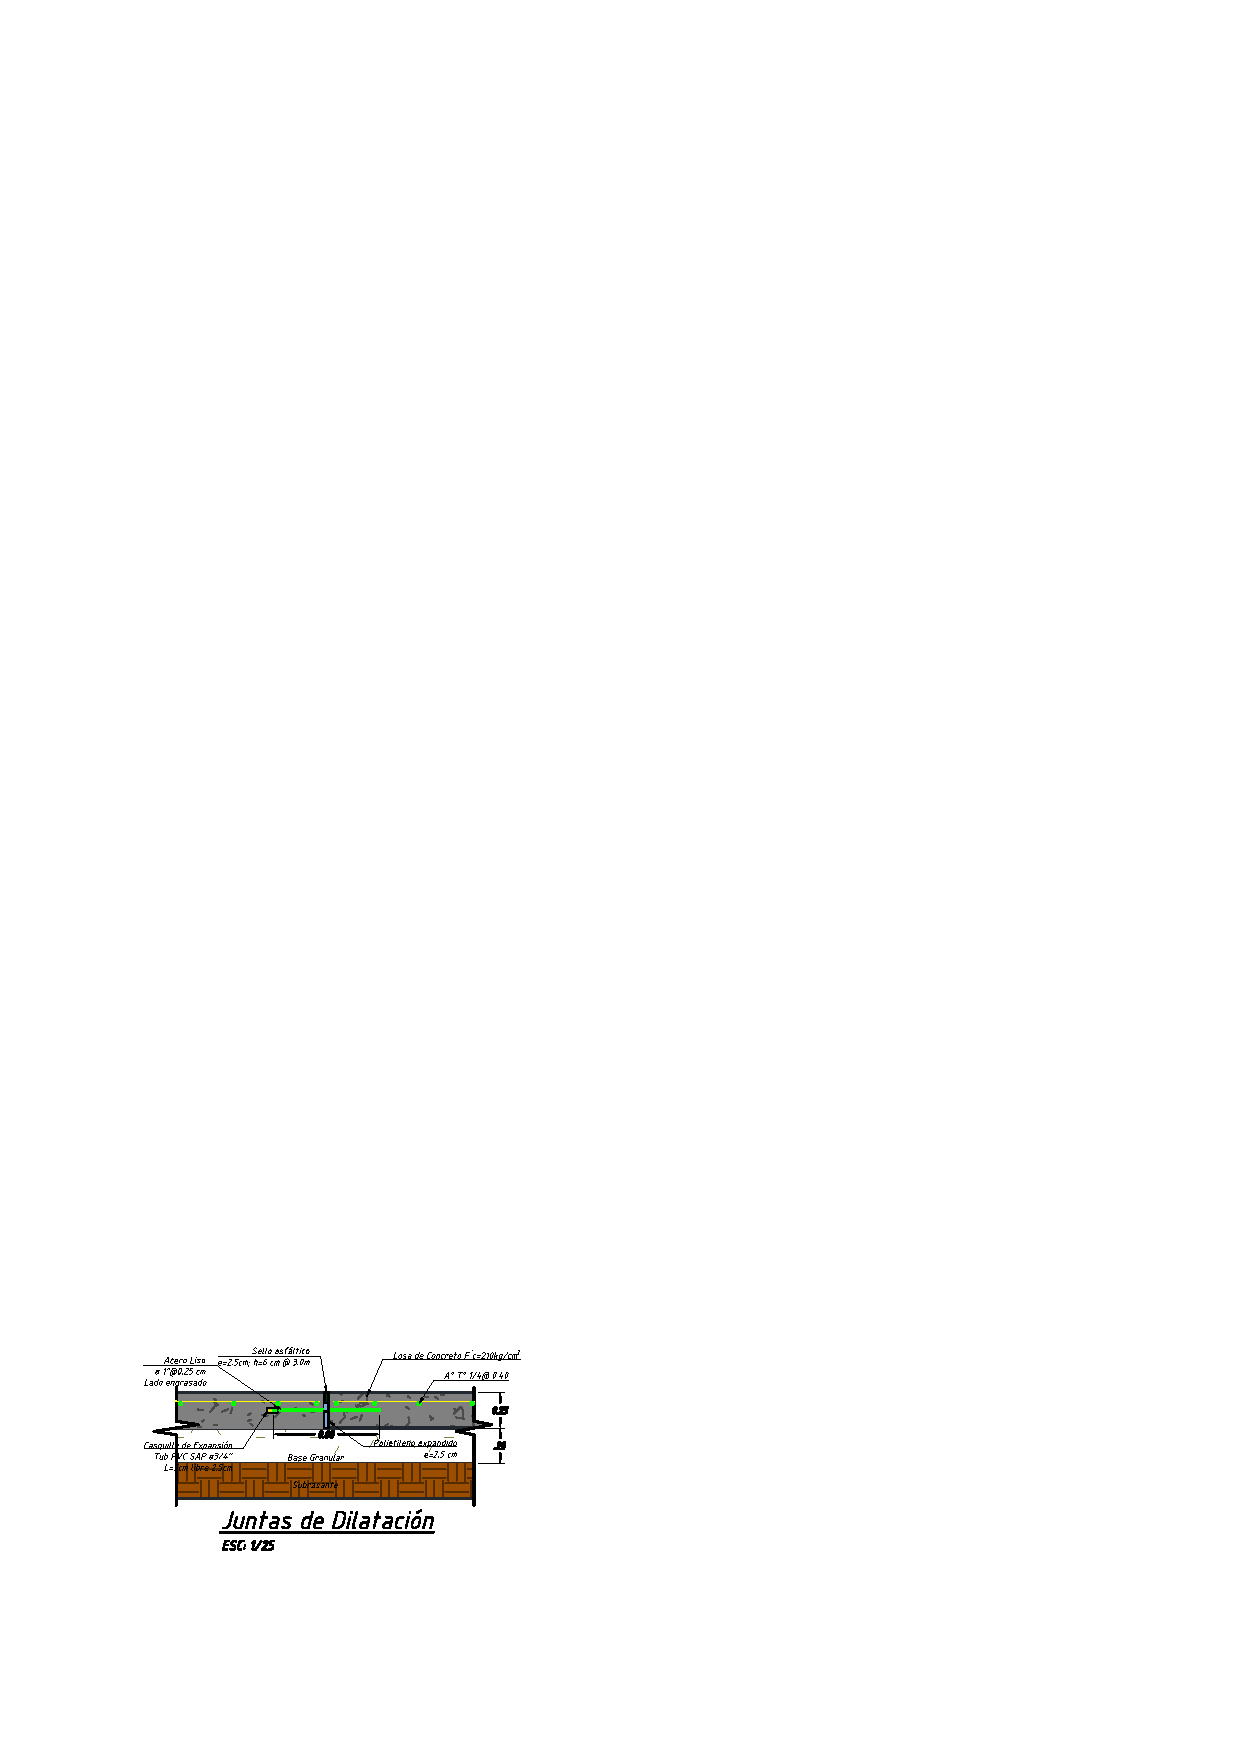
\includegraphics[width=0.8\textwidth]{2.7.pdf}
	\caption[Descripcion corta]{Diseño de juntas transversales de dilatación y demás elementos }
	\label{fig:etiqueta}
	\end{figure}
\end{frame}
%%%%%%%%%%%%%%%%%%%%%%%%%%%%%%% SLIDE 10 %%%%%%%%%%%%%%%%%%%%%%%%%%%%%%%%%
\begin{frame}{Junta transversal}{Método P.C.A}
	\begin{equation}
		L = \frac{2 \cdot S_{c}}{f \cdot Y_{c} \cdot 1.5 }
	\end{equation}
	\begin{block}{Dónde:}
		\begin{itemize}
			\item \(L : \) Espaciamiento entre juntas de Contracción transversal
			\item \(S_{c} : \) Esfuerzo resistente a la tracción del concreto \(1.50 \leq Sc \leq 3.0 kg/cm^{2}\)
			\item \(f :\) Coeficiente de fricción entre el concreto y suelo \(0.50 \leq f \leq 2.5\)
			\item \(Y_{c} :\) Peso especifico del concreto \(Yc= 0.0024 kg/cm^{3}\)
		\end{itemize}
	\end{block}
\end{frame}
%%%%%%%%%%%%%%%%%%%%%%%%%%%%%%% SLIDE 11 %%%%%%%%%%%%%%%%%%%%%%%%%%%%%%%%%
\begin{frame}{Juntas longitudinales}
	\begin{figure}[h]
	\captionsetup{width=1\textwidth}
	\centering
	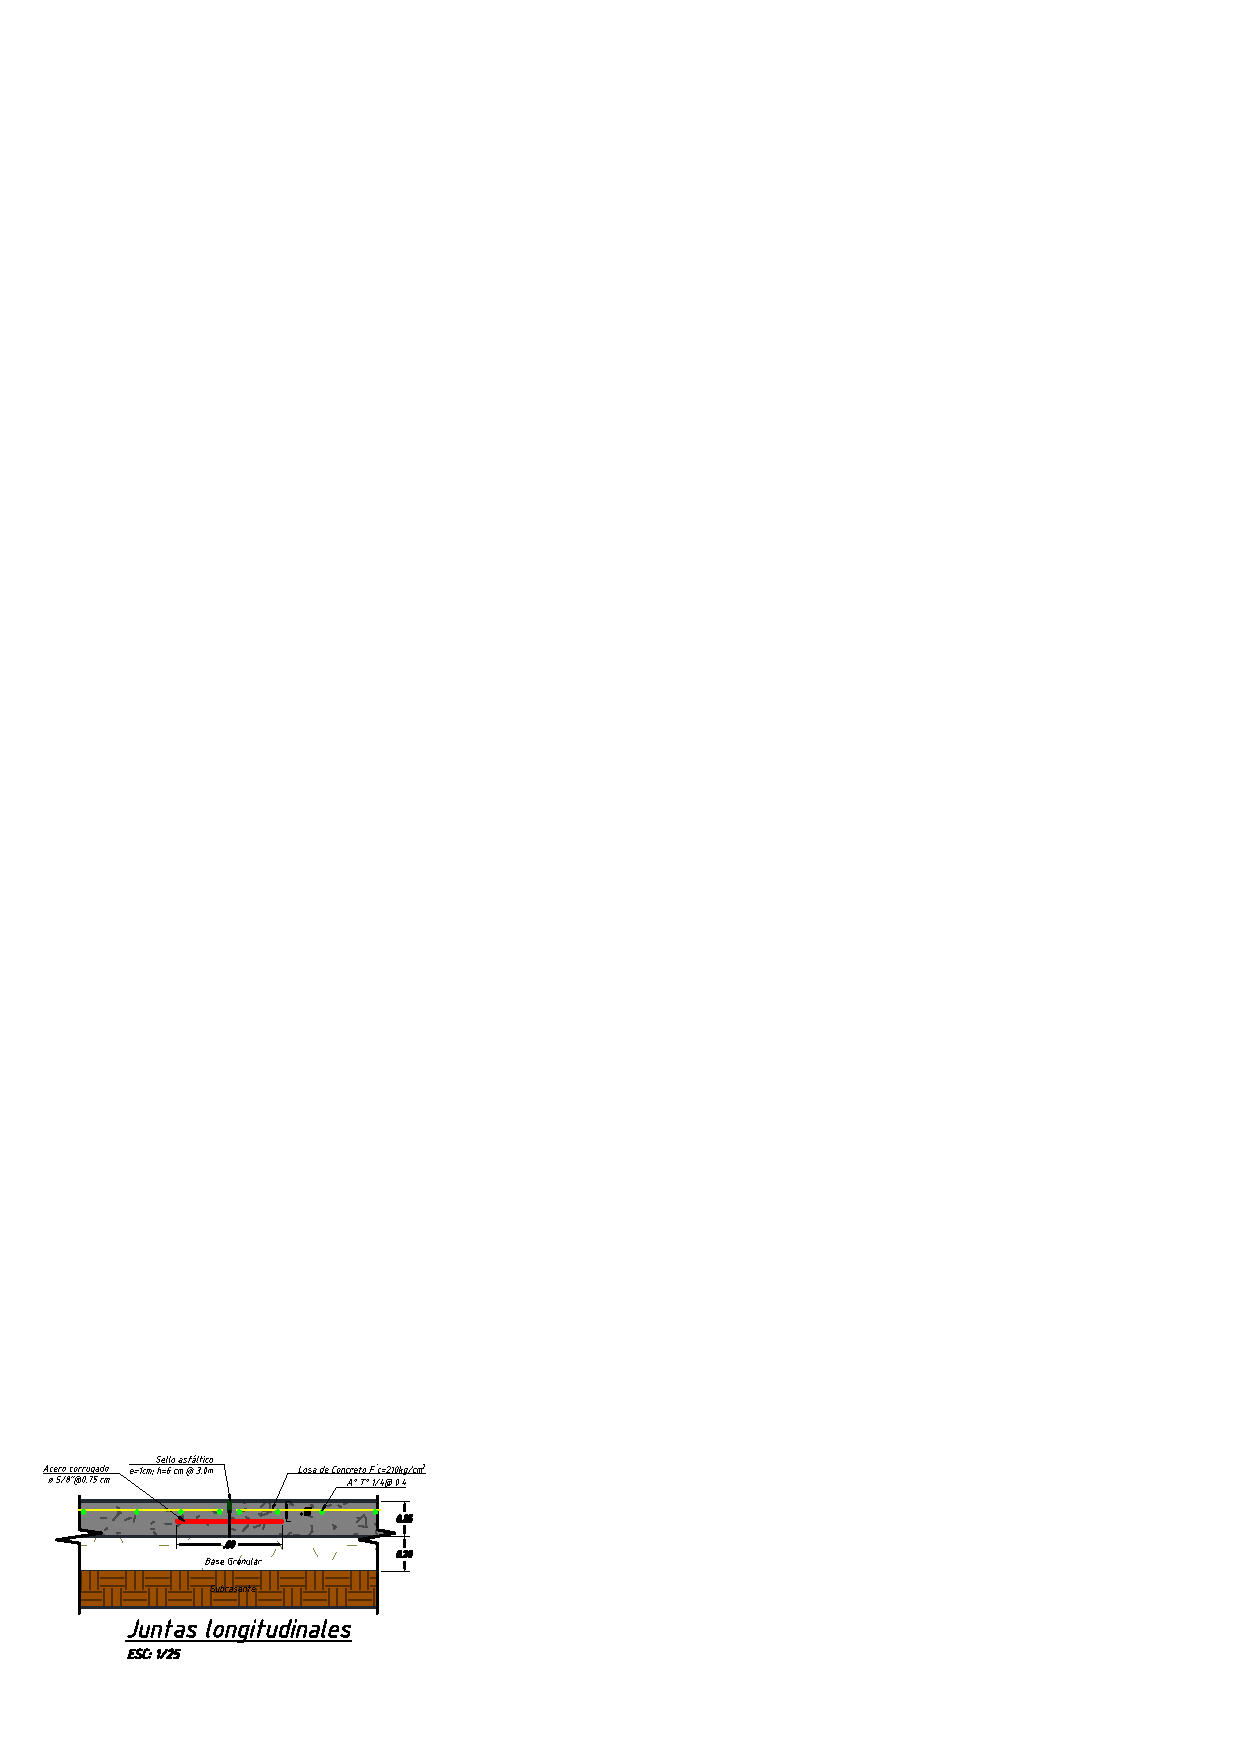
\includegraphics[width=0.8\textwidth]{2.6.pdf}
	\caption[Descripcion corta]{Diseño de juntas longitudinales y demás elementos }
	\label{fig:etiqueta}
	\end{figure}
\end{frame}
%%%%%%%%%%%%%%%%%%%%%%%%%%%%%%% SLIDE 12 %%%%%%%%%%%%%%%%%%%%%%%%%%%%%%%%%
\begin{frame}
	\begin{equation}
		L = \frac{\pi \cdot d^{2} \cdot f_{s}}{4 \cdot a \cdot h \cdot Y_{c} \cdot f}
	\end{equation}
	\begin{block}{Dónde:}
		\begin{itemize}
			\item \(\pi : \) Constante
			\item \(d^{2} : \) Diámetro al cuadrado de la varilla
			\item \(f_{s} :\) Esfuerzo de trabajo del acero \(f_{s} =0.5 \cdot f_{y}\)
			\item \(f :\) Coeficiente de fricción entre paño y suelo; \(f = 2\)
			\item \(L :\) Esfuerzo de trabajo del acero
			\item \(a :\) Ancho de la losa en (cm)
			\item \(h :\) Espesor de losa (cm)
		\end{itemize}
	\end{block}
\end{frame}

%%%%%%%%%%%%%%%%%%%%%%%%%%%%%%% SLIDE 13 %%%%%%%%%%%%%%%%%%%%%%%%%%%%%%%%%

\begin{frame}{Sección típica}
	\begin{figure}[h]
	\captionsetup{width=1\textwidth}
	\centering
	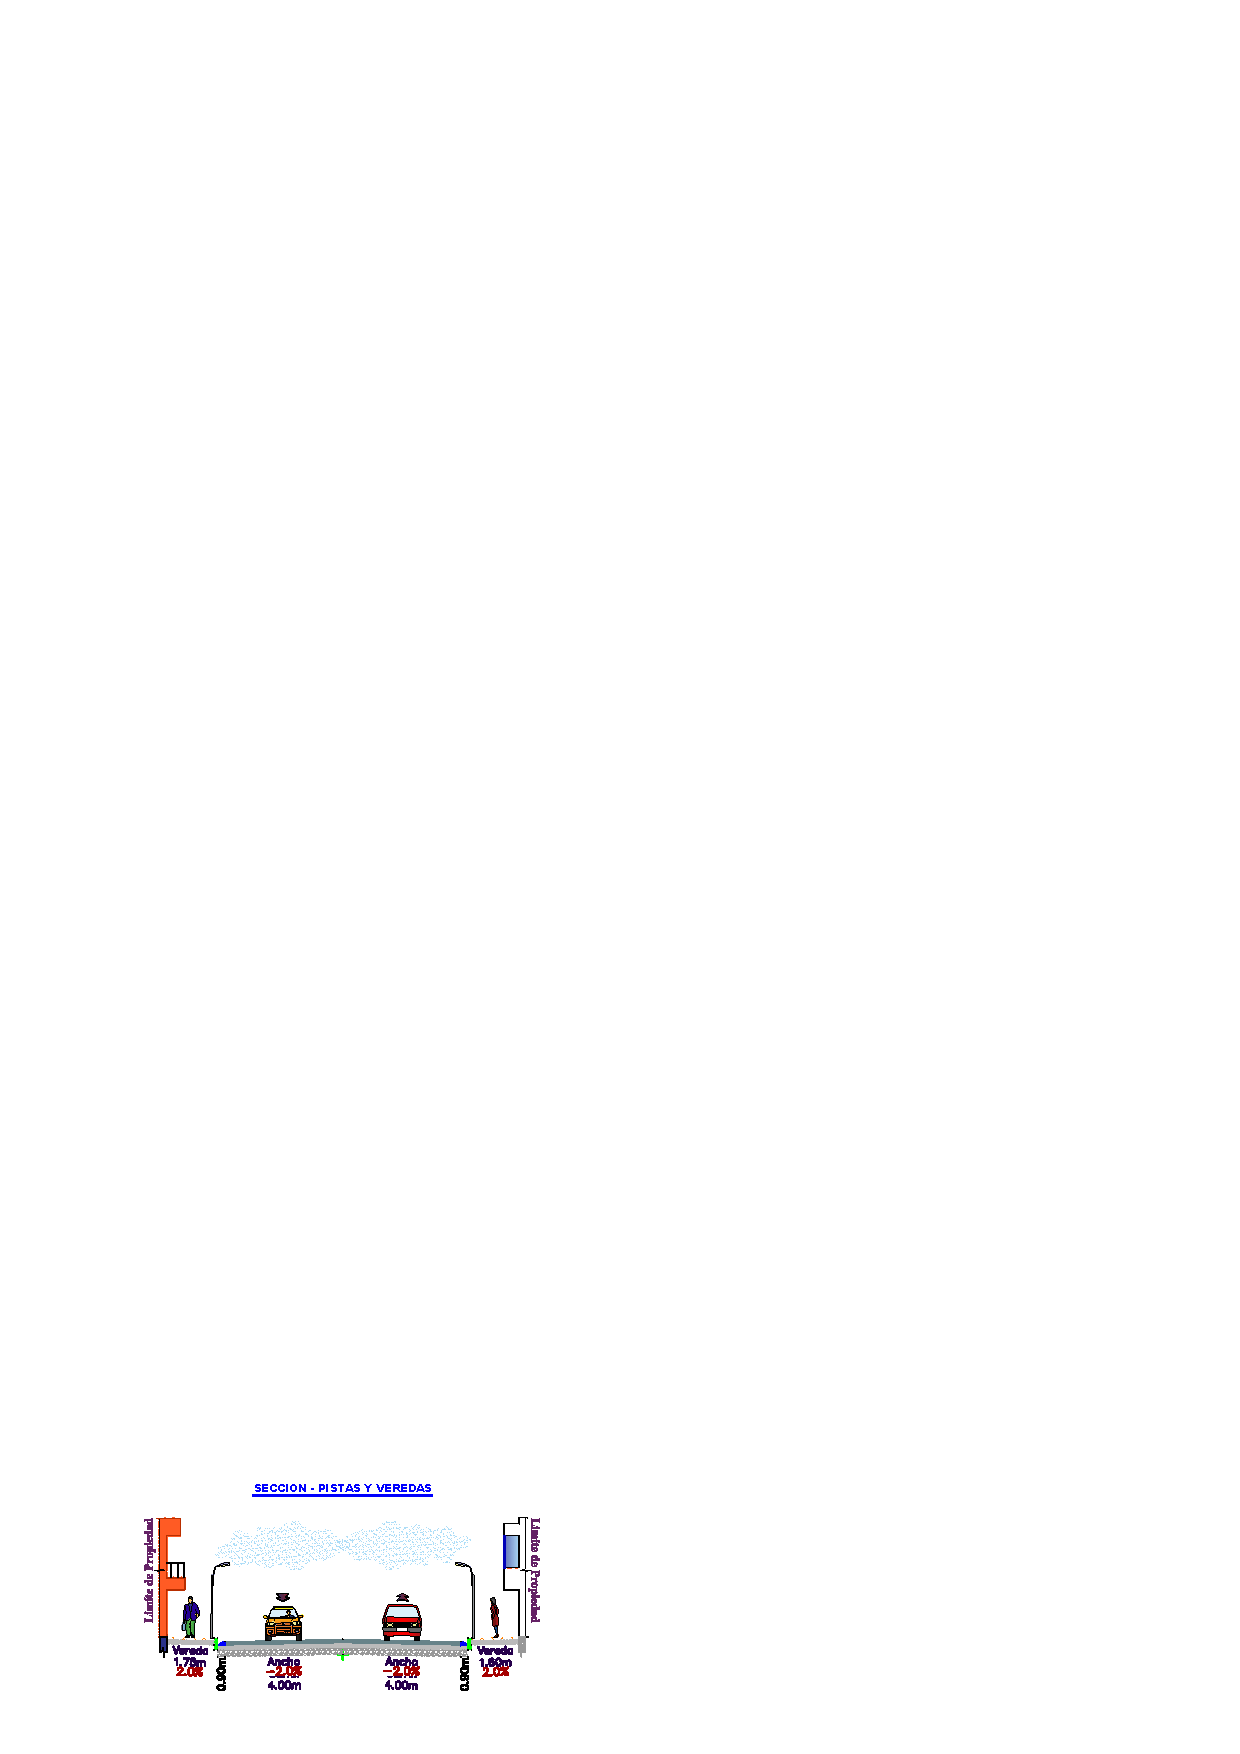
\includegraphics[width=0.8\textwidth]{2.8.pdf}
	\caption[Descripcion corta]{Diseño de sección típica de pistas y veredas }
	\label{fig:etiqueta}
	\end{figure}
\end{frame}

%%%%%%%%%%%%%%%%%%%%%%%%%%%%%%% SLIDE 12 %%%%%%%%%%%%%%%%%%%%%%%%%%%%%%%%%
\begin{frame}{Cálculo de juntas}
	HOLIS
\end{frame}